\documentclass[12pt]{article}
\usepackage[spanish]{babel}
\usepackage[utf8]{inputenc}
\usepackage{csquotes}

% Interlineado 1.5
\usepackage{setspace}
\onehalfspacing

% Fuente Times New Roman
\usepackage{mathptmx}

% Acomodar margenes del documento
\usepackage[a4paper, margin=2cm, top=3cm, headheight=50pt]{geometry}

% Paquetes comunes
\usepackage{graphicx, float}
\usepackage{amsfonts, amssymb, amsmath}
\usepackage{physics, esvect}
\usepackage{enumerate}
\usepackage[colorlinks=true, citecolor=blue]{hyperref}

% Para graficar
\usepackage{pgfplots}
\usepackage{tikz, color}
\usepackage{tikz-3dplot}
\pgfplotsset{width=15cm, compat=1.12}

% Para automatas
\usetikzlibrary{automata, positioning, arrows, calc}
\tikzset{
        ->,  % makes the edges directed
        >=stealth, % makes the arrow heads bold
        shorten >=2pt, shorten <=2pt, % shorten the arrow
        node distance=3cm, % specifies the minimum distance between two nodes. Change if n
        every state/.style={draw=blue!55,very thick,fill=blue!20}, % sets the properties for each ’state’ n
        initial text=$ $, % sets the text that appears on the start arrow
}

% Encabezados
\usepackage{fancyhdr}
\pagestyle{fancy}
\fancyhf{}
\fancyfoot[C]{\thepage}
\fancyhead[L]{
  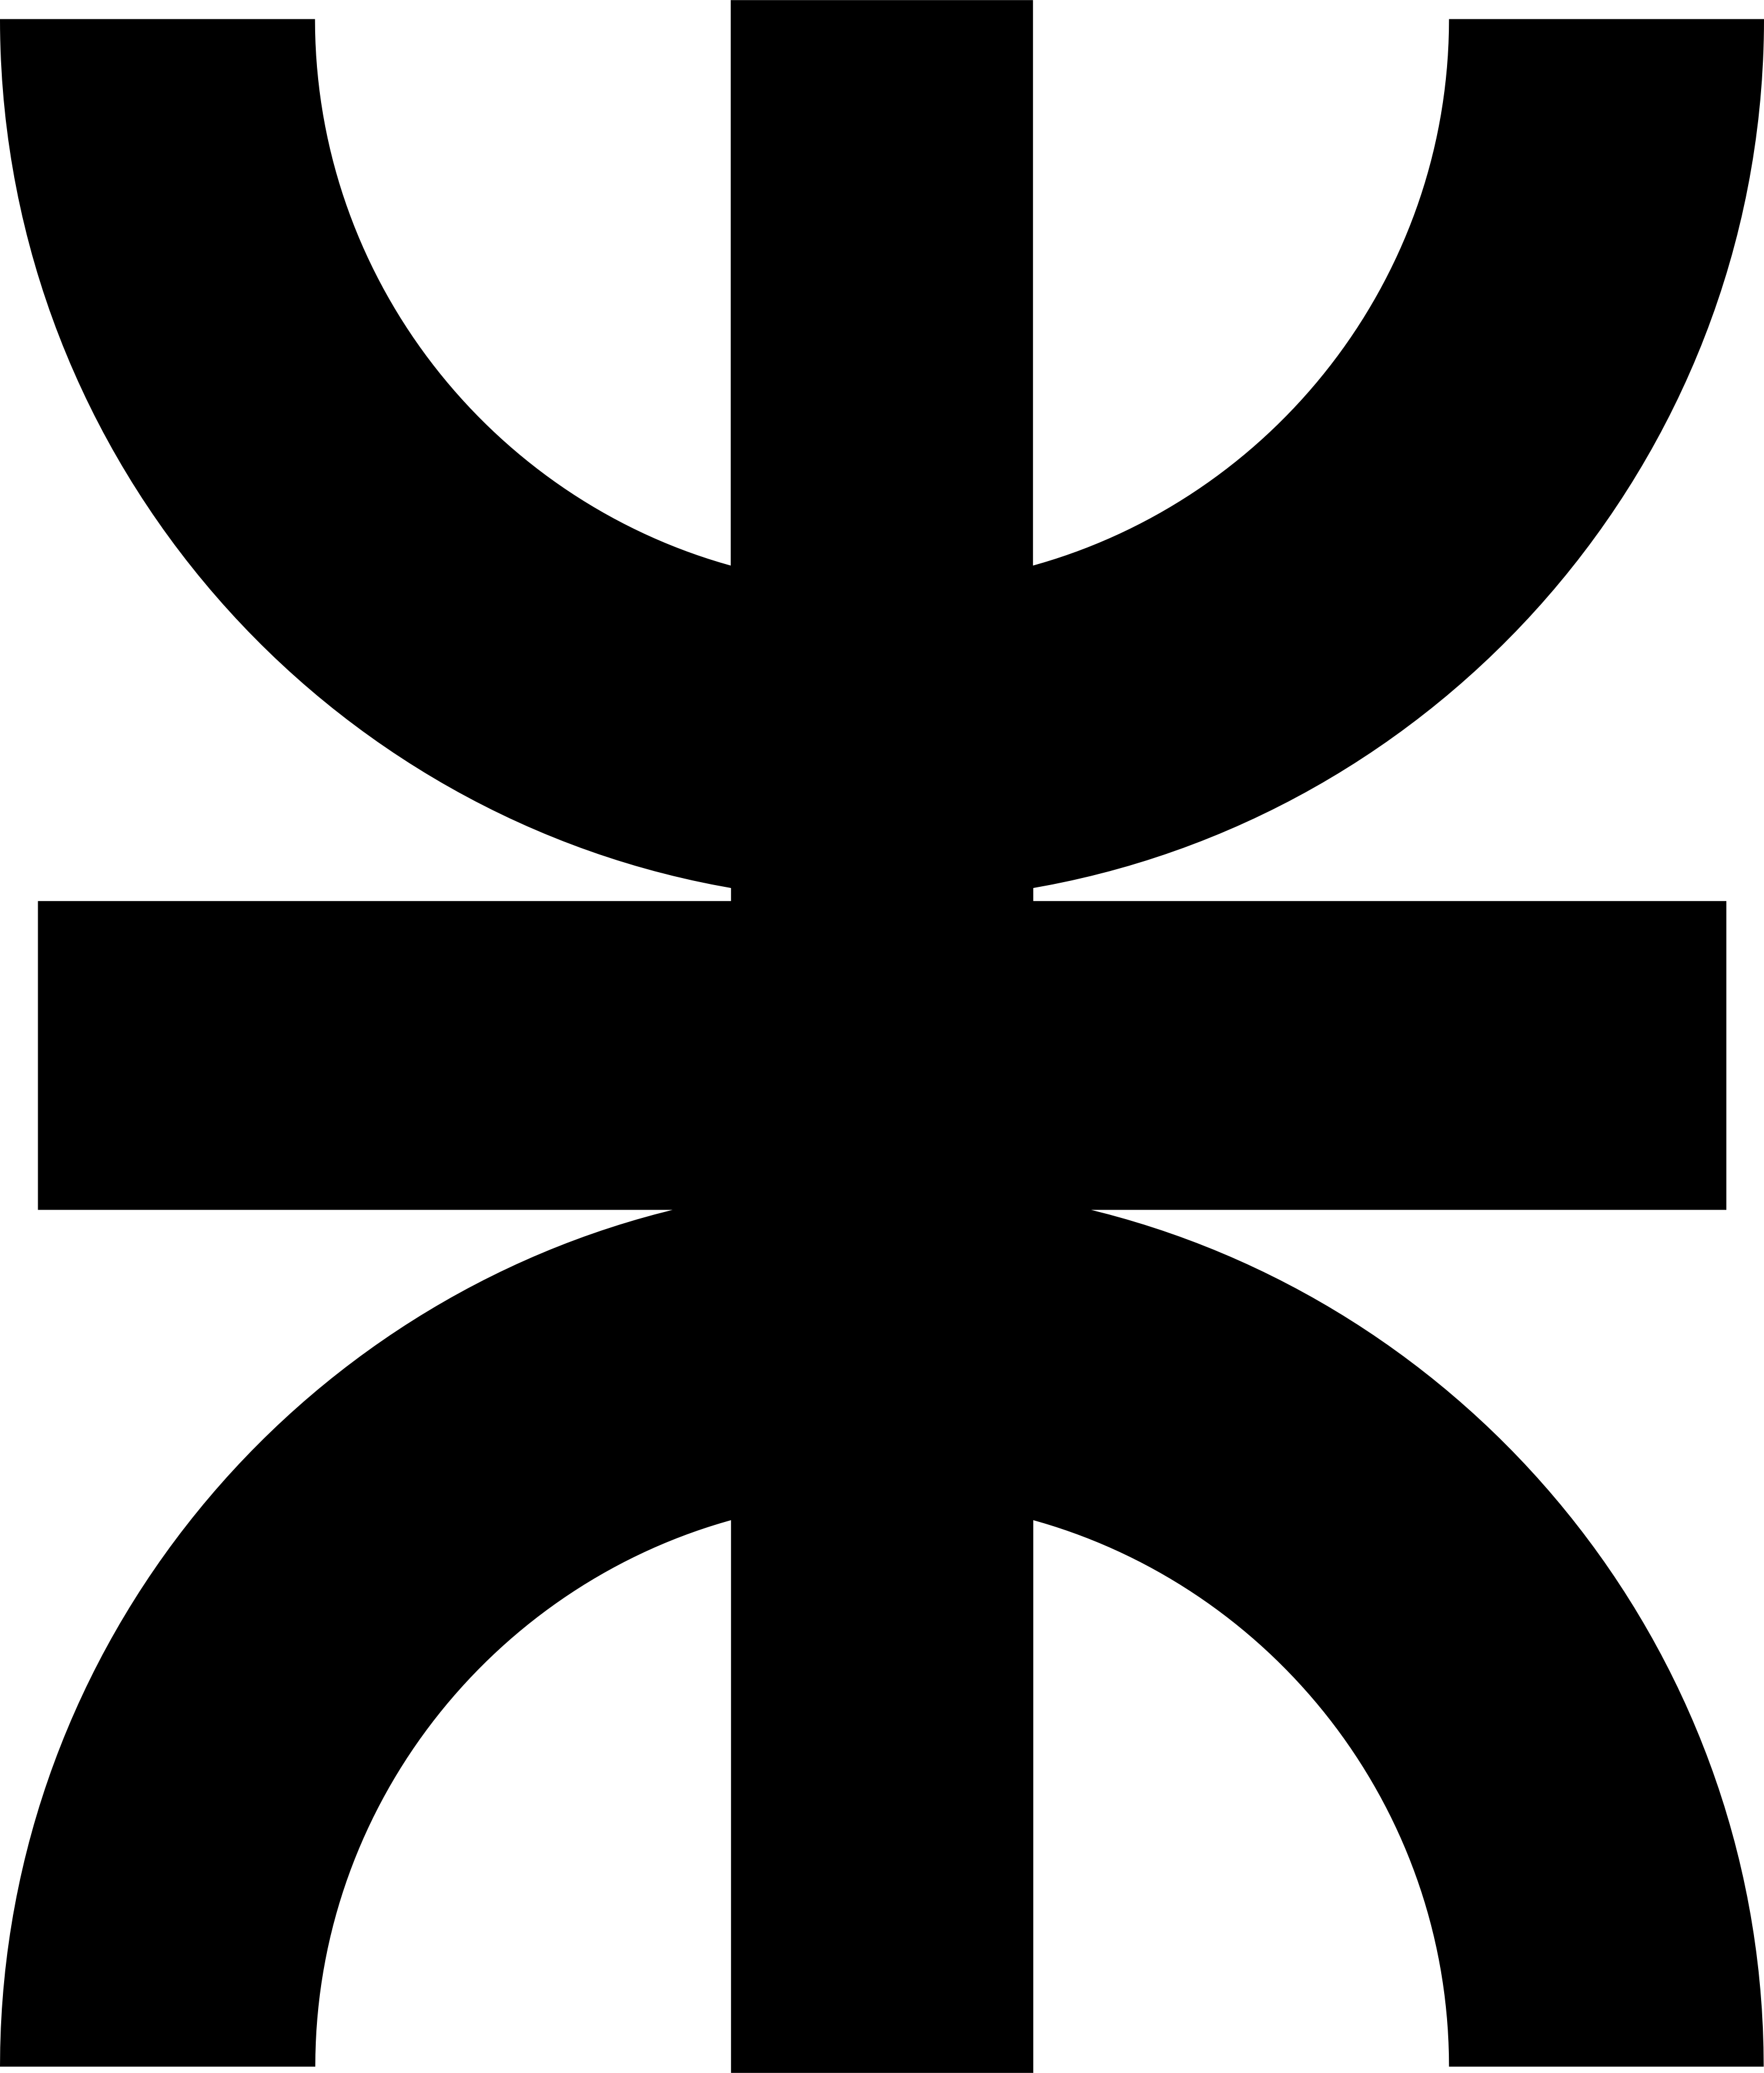
\includegraphics[height=1.2cm]{~/imagenes/logo_utn.png}
  \shortstack[l]{
    {\footnotesize Universidad Tecnológica Nacional} \\
    {\footnotesize Facultad Regional Córdoba} \\
    {\footnotesize Extensión Áulica Bariloche}
  }
}
\fancyhead[C]{
  \shortstack[c]{
    {\footnotesize Sistemas Operativos} \\
    {\footnotesize Resumen para el primer parcial} \\
    {\footnotesize }
  }
}
\fancyhead[R]{
  \shortstack[r]{
    {\footnotesize Profesor: Eduardo Tapia} \\
    {\footnotesize Alumno: Ricardo Nicolás Freccero} \\
    {\footnotesize Fecha: 24/05/2025}
  }
}

% Para bibliografía
\usepackage[backend=biber, style=apa]{biblatex}
\addbibresource{bibliografia.bib}

\begin{document}
\newgeometry{margin=2cm, top=1.5cm}
  \begin{titlepage}
    \centering
    
\includegraphics[width=\linewidth]{~/imagenes/logo_utn_frc.jpg}\\

    \textsc{
      \LARGE Universidad Tecnológica Nacional\\
      \Large Facultad Regional Córdoba - Extensión Áulica Bariloche\\
      \large Ingeniería en Sistemas de Información\\
      Año lectivo 2025\\[0.5cm]
    }

    \rule{\linewidth}{1.0mm}\\[0.4cm]
    \Huge
    \textbf{Sistemas Operativos}\\
    Resumen para el primer parcial\\[0.2cm]
    \LARGE
    Unidades 1, 2 y 3 de la cátedra
    \rule{\linewidth}{1.0mm}\\
    \large
    \begin{flushleft}
      Profesor: Eduardo Tapia

      Ayudante: 

      Fecha: 24/05/2025
    \end{flushleft}

    \vfill
    \begin{flushright}
      Alumno: Ricardo Nicolás Freccero

      Número de legajo: 415753
    \end{flushright}
  \end{titlepage}

  \restoregeometry
  \tableofcontents
  \newpage

  \section{Unidad 1 - Concepto de Sistemas Operativos}
  \subsection{¿Qué es el sistema operativo?}
  Un sistema operativo es un programa que controla la ejecución de aplicaciones y programas. Es quien se encarga de ``conectar'' o ``comunicar'' las apliaciones con el hardeware de la computadora. Se puede considerar que un sistema operativo tiene tres objetivos:

  \begin{itemize}
    \item \textbf{Facilidad de uso.} Un sistema operativo facilita el uso de un computador.

    \item \textbf{Eficiencia.} Un sistema operativo permite que los recursos de un sistema de computación se puedan utilizar de una manera eficiente.

    \item \textbf{Capacidad para evolucionar.} Un sistema operativo se debe construir de tal forma que se puedan desarrollar, probar e introducir nuevas funciones en el sistema sin interferir con su servicio.
  \end{itemize}

  \subsubsection{El sistema operativo como una interaz de usuario/computador}
  El hardware y software que le permiten al usuario acceder y utilizar las aplicaciones y programas de una computadora se pueden ver de forma jerárquica como muestra la Figura \ref{fig:jerarquia-sist-comp}. Al usuario no le suelen interesar los detalles del hardware de la computadora y vé al sistema de computación como un conjunto de aplicaciones. Por otro lado, cada aplicación se puede expresar en un lenguaje de programación y normalmente es desarrollada por un programador. Al programador sí le importan los detalles del hardware, pero no se comunica casi nunca directamente con él ya que suele ser una tarea extremadamente compleja. Para eso existe un \textit{conjunto de programas de sistema} que le permiten al programador comunicarse de una manera mas eficiente con el hardware. El programa de sistema mas importante es el \textbf{sistema operativo} que proporciona una interfáz entre el software y el hardware, actuando como mediador y facilitando el acceso del programador a las utilidades y servicios del sistema.

  \begin{figure}[H]
    \centering
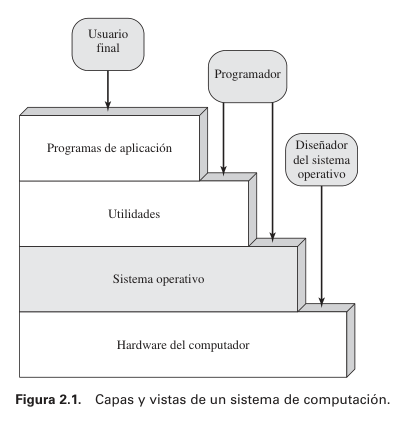
\includegraphics[width=0.4\linewidth]{imagenes/jerarquia-sist-comp.png}
    \caption{Imagen sacada de \parencite{sostallings}. Jerarquía de un sistema de computación.}
    \label{fig:jerarquia-sist-comp}
  \end{figure}

  El sistema operativo proporciona normalmente servicios en las siguientes áreas:
  \begin{itemize}
    \item \textbf{Desarrollo de programas.} Ofrece editores y depuradores para asistir al programador en la creación de programas y aplicaciones.

    \item \textbf{Ejecución de programas.} Se encarga de realizar todos los pasos necesarios para la ejecución de programas en nnombre del usuario.

    \item \textbf{Acceso a dispositivos de E/S.} Facilita el acceso de los programadores a estos dispositivos.

    \item \textbf{Acceso al sistema.} Protege los recursos y los datos,e vitando el uso no autorizado de los ususarios y resolviendo conflictos en el caso de conflico de recursos.

    \item \textbf{Detección y respuesta a errores.} Debe proporcionar una respuesta a cualquier error que pueda surgir de manera que se elimine la condición de error, suponiendo el menor impacto en las aplicaciones que están en ejecución. 

    \item \textbf{Contabilidad.} Recoge estadísticas de uso de los diferentes recursos y monitoriza parámetros de rendimiento. Esta información es útil para anticipar las necesidades de mejoras futuras y para optimizar el sistema a fin de mejorar su rendimiento.
  \end{itemize}

  \subsubsection{El sistema operativo como gestor de recursos}
  El sistema operativo dirige al procesador en el uso de los recursos de la computadora y en el tiempo que debe tomarse para la ejecución de otros programas. Para eso, el sistema operativo cede el control para que el procesador realice sus tareas y luego retoma el control para decirle qué sigue.

  El sistema operativo decide cuándo un programa en ejecución puede utilizar un dispositivo de E/S y controla el acceso y uso de los ficheros, además decide cuánto tiempo debe tomarse cada procesador para la ejecución de un programa.

  \subsubsection{Facilidad de evolución de un sistema operativo}
  Un sistema operativo debe evolucionar en el tiempo por las siguientes razones:
  \begin{itemize}
    \item Actualizacioes de hardware y nuevos tipos de hardware.

    \item Nuevos servicios. (Por ejemplo, si es dificil mantener un buen rendimiento con las herramientas existentes, se pueden añadir al sistema operativo nuevas herramientas de medida y control.)

    \item Resolución de fallos.
  \end{itemize}

  \subsection{Evolución de los sistemas operativos}
  \subsubsection{Procesamiento en serie}
  El programador interactuaba directamente con el hardware de la computadora, que contaba con una consola, luces, interruptores, algún dispositivo de entrada y una impresora; \textit{no existía ningún sistema operativo}. Los programas en código máquina se cargaban a través del dispositivo de entrada y si un error provocaba la parada del programa, las luces indicaban la condición de error. El programador podía examinar los registros del procesador y memoria principal para determinarl la causa del error. Si el programa terminaba de forma normal, la salida se imprimía.

  \subsubsection{Sistemas en lotes sencillos}
  Se empieza a usar un software denominado \textbf{monitor}, que permite que el usuario no tenga que acceder directamente a la máquina. En su lugar, el la computadora recibe una secuencia de trabajos que va a usar el monitor. El monitor de encarga de leer uno a uno cada trabajo y decirle al procesador que los vaya realizando en ese orden.

  \subsubsection{Sistemas en lotes multiprogramados}
  Aún usando un sistema de lotes sencillos, el procesador está haciendo nada la mayoría del tiempo ya que este es mucho mas rápido que los dispositivos de E/S. La computadora pasa mas tiempo buscando la información que tiene que procesar el procesador que procesando esa información. Lo que se puede hacer entonces es que mientras se está esperando por la E/S, se le puede asignar al procesador otro trabajo que no esté esperando por una operación de E/S. 

  \begin{figure}[H]
    \centering
    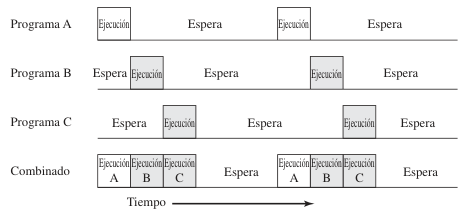
\includegraphics[width=0.5\linewidth]{imagenes/multiprogramacion.png}
    \caption{Imagen sacada de \parencite{sostallings}. Ejemplo de multiprogramación con tres programas.}
    \label{fig:multiprog}
  \end{figure}
  

  \subsubsection{Sistemas de tiempo compartido}
  Son sistemas que comparten el tiempo de programación entre múltiples usuarios.

  \subsection{Desarrollos que llevaron a los sistemas operativos modernos}
  \subsubsection{Arquitectura micronúcleo o microkernel}
  Antes, la mayoría de los sistemas operativos estaban formados por \textbf{núcleos monolíticos}. Estos núcleos proporcinaban la mayoría de las funcionalidades consideradas propias del sistema operativo, incluyendo planificación, los sistemas de ficheros, las redes, los controladores de dispositivos, la gestióno de memoria, etc. Una \textbf{arquitectura microkernel} asigna sólo unas pocas funciones esenciales al kernel, incluyendo los espacios de almacenamiento, comunicación entre procesos, y planificación básica.

  \subsubsection{Multithreading}
  Es una técnica en la cual un proceso, ejecutando una aplicación, se divide en una serie de \textit{hilos} o \textit{threads}.
  \begin{itemize}
    \item \textbf{Thread o hilo.} Es una unidad de trabajo. Incluye el contexto del procesador (que contiene el contador del programa y el puntero de pila) y su propia área de datos para una pila (para posibilitar el salto a subrutinas). Un hilo se ejecuta secuencialmente y se puede interrumpir para dar paso a otro hilo.

    \item \textbf{Proceso.} Es una colección de uno o más hilos y sus recursos de sistema asociados. Es un programa en ejecución.
  \end{itemize}

  Esta técnica es útil para aplicaciones que llevan a cabo tareas que no necesitan correrse en serie, es decir, que se pueden ejecutar en simultáneo.

  \subsubsection{Multiprocesamiento simétrico (SMP)}
  Se refiere a la arquitectura del hardware de la computadora y al comportamiento del sistema operativo que explota dicha arquitectura. Tiene las siguientes características:
  \begin{itemize}
    \item Tiene múltiples procesadores.

    \item Los procosadores comparten las mismas utilidades de momeira principal y de E/S.

    \item Todos los procesadores pueden realizar las mismas funciones.
  \end{itemize}

  El sistema operativo de un SMP planifica procesos o hilos a través de todos los procesadores.
  \begin{figure}[H]
    \centering
    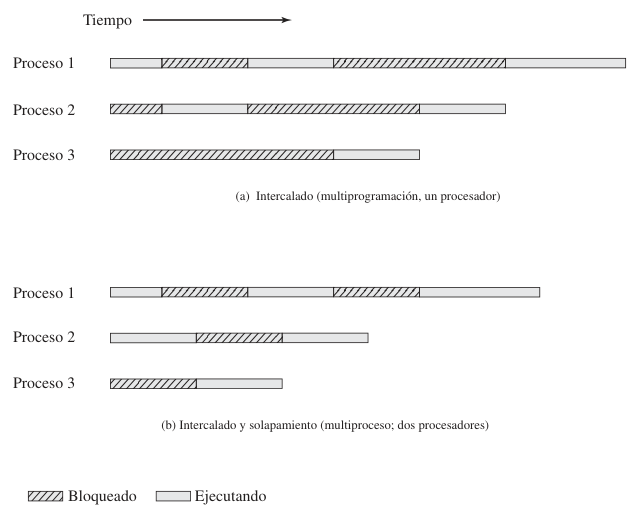
\includegraphics[width=0.7\linewidth]{imagenes/smp-vs-no-smp.png}
    \caption{Imagen sacada de \parencite{sostallings}. Multiprogramación y multiproceso.}
    \label{fig:smp}
  \end{figure}
  
  \subsubsection{Sistema operativo distribuído}
  Da la ilusión de tener un solo espacio de memoria principal y un solo espacio de memoria secundario, cuando tenemos un ``cluster'' de computadoras (varias computadoras que operan como si fuese una sola).

  \subsubsection{Diseño orientado a objetos}
  Introduce una disciplina al proceso de añadir extensiones modulares a un pequeño núcleo. Permite a los programadores personalizar un sistema operativo sin eliminar la integridad del sistema.

  \subsection{Sistemas UNIX tradicionales}
  UNIX es un sistema operativo que se desarrollo inicialmente en los laboratorios de Bell y se hizo operacional en 1970. En la figura \ref{fig:arq-unix} se puede ver la arquitectura general de UNIX.

  \begin{figure}[H]
    \centering
    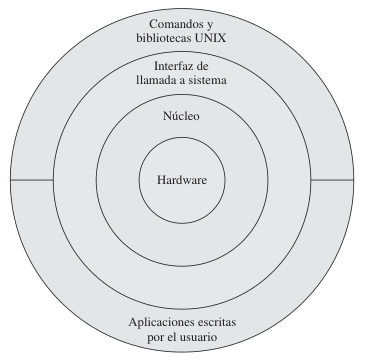
\includegraphics[width=0.6\linewidth]{imagenes/arquitectura-unix.png}
    \caption{Imagen sacad de \parencite{sostallings}. Arquitectura general de UNIX.}
    \label{fig:arq-unix}
  \end{figure}

  \subsection{Linux}
  Linux comenzó como una variante UNIX. Linus Torvalds, un estudiante finlandés de informática, escribió la versión inicial. Linux es un sistema UNIX completo de software libre (cualquier persona puede ver y modificar el código fuente).

  La mayoría de los núcleos de Linux son monolíticos.  Aunque no usa la técnica de microkernel, logra muchas de las ventajas potenciales de esta por medio de su arquitectura modular particular. Linux está estructurado como una colección de módulos, algunos de los cuales pueden cargarse y descargarse automáticamente bajo demanda. Estos bloques se denominan \textbf{módulos cargables}.

  Los módulos cargables de Linux tienen dos características importantes:
  \begin{itemize}
    \item \textbf{Enlace dinámico}. Un módulo de núcleo puede cargarse y enlazarase al núcleo mientras el núcleo está en memoria y ejecutándose. Un módulo también puede desenlazarase y eliminarse de la memoria en cualquier momento.

    \item \textbf{Módulos apilables}. Los módulos se gestionan como una jerarquía. Cuando un módulo superior en la jerarquía referencia a un módulo inferior, el primero actúa como módulo cliente y el segundo como biblioteca.
  \end{itemize}

  \section{Unidad 2 - Administración y Gestión de Archivos}
  Los \textbf{archivos} son unidades logicas de informacion que pueden ser leidas o creadas por los procesos. La informacion que se almacena en los archivos debe ser persistente. Un archivo debe desaparecer solo cuando su propietario lo remueve de manera explicita.

  Los archivos son administrados por el sistema operativo. La parte del sistema operativo que trata con los archivos se conoce como \textbf{sistema de archivos}.

  \subsection{Archivos}
  Los archivos proporcionan una manera de almacenar informacion en el disco y leerla despues. Cuando un proceso crea un archivo le proporciona un nombre. Cuando el proceso termina, el archivo sigue existiendo y puede ser utilizado por otros procesos mediante su nombre.

  Algunos sistemas de archivos, como el de UNIX, diferencian las letras mayusculas de las minusculas, mientras que otros no.

  Existen varios sistemas de archivos que vamos a analizar mas adelante. Por ahora solo vamos a decir que Windows 95 y 98 usan el sistema de archivos \textbf{FAT-16}. Windows 98 extendio FAT-16 e introdujo \textbf{FAT-32} pero estos dos sistemas son bastante similares. Las versiones mas nuevas de Windows admiten ambos sistemas FAT, que en realidad ya son obsoletos, pero tienen un sistema de archivos nativo que se conoce como \textbf{NTFS}.

  Muchos sistemas operativos aceptan nombres de archivos en dos partes, separadas por un punto. La parte que va despues del punto se conoce como la \textbf{extension del archivo} y suele indicar algo acerca de la naturaleza de ese archivo.
  
  En algunos sistemas (como UNIX) las extensiones de archivo son solo convenciones y no son impuestas por el sistema operativo. Funcionan mas como un recordatorio para el propietario que como un medio para transportar informacion a la computadora. Sin embargo, en otros sistemas (como Windows) éste es consciente de las extensiones y les asigna significado. Los usuarios pueden registrar extensiones y asignar programas a cada una de manera que cuando se le hace doble click al nombre del archivo, el programa asignado a su extension se inicia con ese archivo como parametro.

  \subsubsection{Estructura de archivos}
  Los archivos se pueden estructurar de varias formas:
  \begin{itemize}
    \item \textbf{Secuencias de byte sin estructura.} El sistema operativo no sabe, ni le importa que hay en el archivo. Esto provee la maxima flexibilidad ya que los programas de usuario pueden colocar cualquier cosa que quieran en sus archivos y denominarlos de cualquier manera conveniente.

    \item \textbf{Secuencia de registros.} Un archivo es una secuencia de registros de longitud fija, cada uno con cierta estructura interna. Estos sistemas se usaban cuando todavia se utilizaban las tarjetas perforadas de 80 columnas, de manera que cada registro consistia de 80 caracteres, simulando la tarjeta.

    \item \textbf{Arbol.} Un archivo consiste en un arbol de registros, donde no todos son necesariamente de la misma longitud; cada uno de llos contiene un campo llave en una posicion fija dentro del registro. El arbol se ordena con base en el campo llave para permitir una busqueda rapida por una llave especifica.
  \end{itemize} 

  \begin{figure}[H]
    \centering
    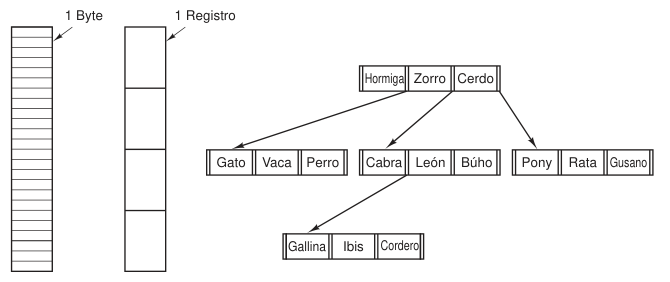
\includegraphics[width=\linewidth]{imagenes/tipos-de-archivos.png}
    \caption{Imagen sacada de \parencite{tanenbaum}. Tres tipos de archivos.}
    \label{fig:tipos-de-archivos}
  \end{figure}

  \subsubsection{Tipos de archivos}
  Muchos sistemas operativos soportan varios tipos de archivos. Por ejemplo, UNIX y Windows tienen archivos y directorios regulares. UNIX también tiene archivos especiales de caracteres y de bloques. Los \textbf{archivos regulares} son los que contienen información del usuario. Los \textbf{directorios} son sistemas de archivos para mantener la estructura del sistema de archivos. Los \textbf{archivos especiales de caracteres} se relacionan con la E/S y se utilizan para modelar dispositivos de E/S en serie. Los \textbf{archivos especiales de bloques} se utilizan para modelar discos.

  Por lo general, los \textbf{archivos regulares} son archivos ASCII o binarios. Los archivos ASCII consisten en líneas de texto, se pueden mostrar e imprimir como están, y se pueden editar con cualquier editor de texto. Los archivos binarios tienen código binario y una cierta estructura interna conocida para los programas que los utilizan. La Figura \ref{fig:archivos-binarios} muestra dos archivos binarios de las primeras versiones de UNIX. El primero es un archivo binario ejecutable. El segundo es una colección de procedimientos (módulos) de biblioteca compilados, pero no enlazados.

  \begin{figure}[H]
    \centering
    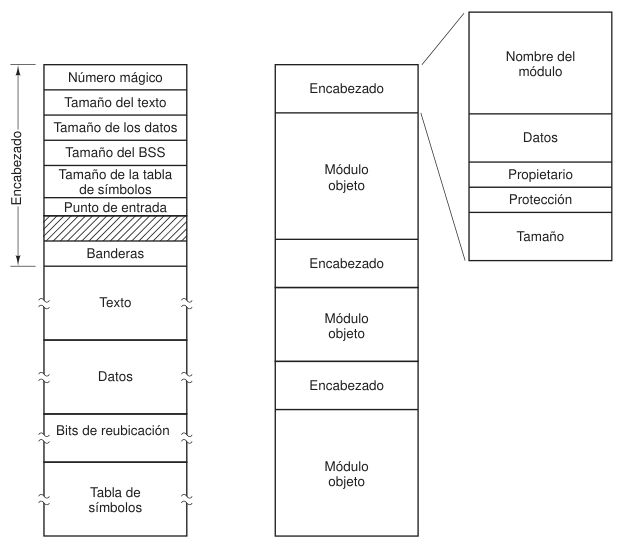
\includegraphics[width=\linewidth]{imagenes/archivos-binarios.png}
    \caption{Imagen sacada de \parencite{tanenbaum}. Dos archivos binarios distintos.}
    \label{fig:archivos-binarios}
  \end{figure}

  \subsubsection{Acceso a archivos}
  Los primeros sistemas operativos proporcionaban sólo un tipo de acceso: \textbf{acceso secuencial}. En estos sistemas, sólo se podían leer los bytes en orden secuencial, pero no se podía saltar entre bytes.

  Mas adelante se crearon los \textbf{archivos de acceso aleatorio} en los que se pueden leer sus bytes en cualquier orden. En estos se pueden usar los métodos \verb|seek| (para establecer la posición desde la que se quiere comenzar a leer) y \verb|read| (para comenzar a leer de manera secuencial desde la posición actual).

  \subsubsection{Atributos de archivos}
  Todo archivo tiene un nombre y sus datos. Además, todos los sistemas operativos asoian otra información con cada archivo. A estos elementos adicionales se los conoce como \textbf{atributos}. A continuación se muestra una tabla con varios atributos, aunque no son todos, que \textit{pueden} tener los archivos en un sistema operativo.

  \begin{figure}[H]
    \centering
    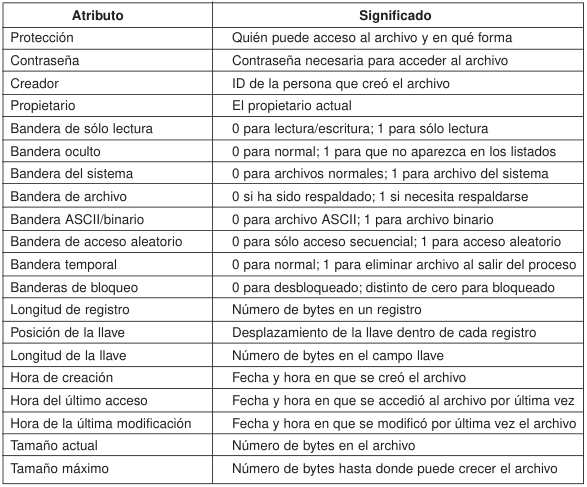
\includegraphics[width=0.8\linewidth]{imagenes/atributos-archivos.png}
    \caption{Imagen sacada de \parencite{tanenbaum}. Algunos atributos de archivos.}
    \label{fig:atributos-archivos}
  \end{figure}
  
  \subsubsection{Operaciones de archivos}
  Las llamadas al sistema (system calls) mas comunes relacionadas con los archivos son las siguientes:
  \begin{enumerate}[1.]
    \item \verb|Create|. El archivo se crea sin datos.

    \item \verb|Delete|. Se elimina el archivo, liberando el espacio en disco.

    \item \verb|Open|. Se llevan los atributos y la lista de direcciones de disco a memoria principal para tener acceso rápido al archivo.

    \item \verb|Close|. Se libera el espacio que ocupaba el archivo en la memoria principal.

    \item \verb|Read|. Se leen los datos del archivo desde la posición actual.

    \item \verb|Write|. Se escriben datos en el archivo desde la posición actual.

    \item \verb|Append|. Se escriben datos al final del archivo.

    \item \verb|Seek|. Se modifica la posición actual del puntero del archivo.

    \item \verb|Get attributes|. Se obtienen los atributos de un archivo.

    \item \verb|Set attributes|. Algunos de los atributos los puede establecer el usuario y se pueden modificar después de haber creado el archivo.

    \item \verb|Rename|. Se cambia el nombre del archivo.
  \end{enumerate}

  \subsection{Directorios}
  Para llevar el registro de los archivos, los sistemas de archivos por lo general tiene \textbf{directorios}, que en muchos sistemas también son archivos.

  \subsubsection{Sistemas de direcorios de un solo nivel}
  La forma más simple de un sistema de directorios es tener un directorio que contenga todos los archivos. Como si en nuestra computadora solo tuviesemos una sola carpeta, y en ella existan todos los archivos que necesitamos.

  \subsubsection{Sistemas de directorios jerárquicos}
  El sistema anterior es útil para aplicaciones simples, pero nos podemos imaginar que sería un caos si fuese el caso de nuestra computadora. Lo que se hace ahora es tener un \textbf{árbol de directorios}. De esta manera, existe un directorio raíz (que en UNIX suele ser ``/'') del que se desprenden tantos directorios como quiera el usuario para agrupar los archivos de la forma mas conveniente.

  \subsubsection{Nombres de rutas}
  Al tener el File System organizado como un árbol de directorios, se necesita cierta forma de especificar los nombres de los archivos y existen dos métodos para lograr esto.
  \begin{itemize}
    \item \textbf{Nombre de ruta absoluto.} Consiste en usar el camino desde el directorio raíz hasta el archivo. Un ejemplo en Linux es \verb|/home/ricman/uni/apuntes/sop/parcial1/resumen.pdf|, que es la dirección en donde se encuentra este documento.

    \item \textbf{Nombre de ruta relativa.} Consiste en nombrar al archivo siguiendo el camino desde el \textbf{directorio actual}, que es el directorio de trabajo, en el que está parado el usuario, hasta el archivo deseado. Por ejemplo, si nuestro directorio actual es \verb|/home/ricman/uni/|, y quiero referenciar este archivo, su nombre de ruta relativa sería \verb|apuntes/sop/parcial1/resumen.pdf|.
  \end{itemize}

  La mayoría de sistemas operativos que proporcionan un sistema de directorios jerárquico tienen dos entradas especiales en cada directorio ``.''(punto) y ``..''(puntopunto). \textit{Punto} se refiere al directorio actual; \textit{puntopunto} se refiere al directorioi padre del directorio actual. Esto es útil cuando queremos acceder a archivos que se encuentran en el directorio padre del directorio actual, pero no queremos usar una ruta absoluta para acceder a él.

  El directorio \textit{punto} suele ser utilizado cuando, por ejemplo, queremos copiar algún archivo de un directorio externo al directorio actual. Para eso podemos usar el comando \verb|cp| (copy) y pasarle primero el nombre del archivo que queremos copiar y luego el directorio actual usando \textit{punto}.

  \verb|cp /home/ricman/uni/apuntes/hola.txt .|

  Lo anterior es lo mismo que decir 

  \verb|cp /home/ricman/uni/apuntes/hola.txt /home/ricman/uni/apuntes/sop/parcial1/|

  \subsubsection{Operaciones de directorios}
  Al igual que con los archivos, podemos realizar varias operaciones con los directorios. En el libro \parencite{tanenbaum} se nombran unas operaciones que me parece que son viejisimas y no las vamos a usar en la cátedra. Pongo a continuación las que yo considero que son equivalentes y sí vamos a usar en la cátedra:
  \begin{enumerate}[1.]
    \item \verb|mkdir| (MaKe DIRectory). Crea un directorio vacío, excepto por \textit{punto} y \textit{puntopunto} que el sistema coloca de manera automática.

    \item \verb|rm -r| (RemoVe). En realidad \verb|rm| es un comando que se utiliza para borrar archivos, pero al pasarle el argumento \verb|-r| es capaz de borrar directorios.

    \item \verb|cd| (Change Directory). Este comando los usamos para movernos entre los directorios del File System.

    \item \verb|mv| (MoVe). Al igual que \verb|rm|, el comando \verb|mv| se usa para ``mover'' archivos o directorios de un lugar a otro dentro del File System. Esto lo hace tomando como primer parámetro el archivo o directorio que deseamos mover, y como segundo el lugar a donde lo queremos mover, entonces crea una copia del archivo en la dirección especificada y borra el original. Esto lo podemos usar para \textit{renombrar} directorios si le decimos que lo mueva desde un directorio hacia el mismo lugar pero con otro nombre. Por ejemplo \verb|mv /home/ricman/uni/ /home/ricman/versi| renombra el directorio ``uni'' como ``versi''.

    \item \verb|ln| (LiNk). Crea un \textbf{vínculo} desde un archivo existente hasta el nombre especificado por la ruta. De esta forma, el mismo archivo puede aparecer en varios directorios. 
  \end{enumerate}

  Una variante sobre la idea de vincular archivos es el \textbf{vínculo simbólico}. En vez de tener dos nombres que apunten a la misma estructura de datos interna que representa un archivo (como hace un vínculo), se puede crear un nombre que apunte a un archivo que nombre a otro.

  \subsection{Implementación de File Systems}
  Ya vimos qué son los archivos y cuáles son sus propiedades, y qué son los directorios y cuáes son sus propiedades. Ahora vamos a ver cómo se almacenan, cómo se administra el espacio en el disco y cómo hacer que todo funcione con eficiencia y confiabilidad.

  \subsubsection{Distribución del sistema de archivos}
  Los sistemas de archivos se alamacenan en discos. La mayoría de discos se pueden dividir en una o más particiones, con sistemas de archivos independientes en cada partición. El sector 0 del disco se conoce como el \textbf{MBR} (\textit{Master Boot Record}) y se utiliza para arrancar la computadora. El final del MBR contiene la tabla de particiones, la cual proporciona las direcciones de inicio y fin de cada partición. Una de las particiones en la tabla se marca como activa. Cuando se arranca la computadora, el BIOS lee y ejecuta el MBR. Lo primero que hace el programa MBR es localizar la partición activa, leer su primero bloque, conocido como el \textbf{bloque de arranque}, y ejecutarlo. El programa en el bloque de arranque carga el sistema operativo contenido en esa partición. 

  \begin{figure}[H]
    \centering
    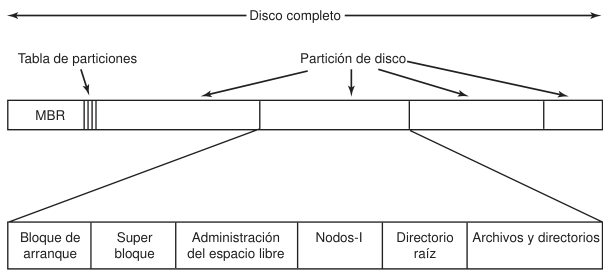
\includegraphics[width=\linewidth]{imagenes/distro-sistema-archivos.png}
    \caption{Imagen sacada de \parencite{tanenbaum}. Una posible distribución del sistema de archivos.}
    \label{fig:distro-file-system}
  \end{figure}
  
  \subsubsection{Implementación de archivos}
  Existen varias formas para implementar el almacenamiento de archivos.

  \paragraph{Asignación contigua}\mbox{}\\
  El esquema de asignación más simple es almacenar cada archivo como una serie contigua de bloques de disco. Así, en un disco con bloques de 1 KB, a un archivo de 50 KB se le asignarían 50 bloques consecutivos.

  Este sistema es facil de implementar ya que solo hay que saber dónde empieza y dónde termina cada archivo, y el rendimiento de lectura es excelente ya que se lee secuencialmente. Sin embargo, tiene una gran desventaja debido a que con el transcurso del tiempo, los discos se fragmentan. Podemos ver en la siguiente figura que a medida que vamos eliminando o modificando los archivos, empiezan a aparecer espacios vacíos entre archivos. Y si después queremos reutilizar ese espacio tendríamos que estar viendo que el archivo que queramos meter ahí entre justo en el hueco para no desaprovechar espacio. Otra opción sería compactar todo el espacio, moviendo todos los archivos para volver a dejar el espacio libre al fondo del disco. Ambas opciones son extremadamente costosas y no termina siendo ``worth''.

  \begin{figure}[H]
    \centering
    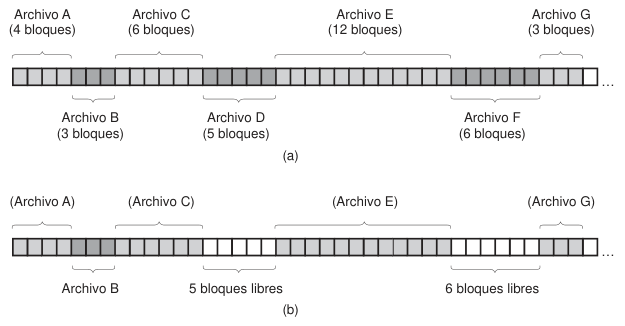
\includegraphics[width=0.8\linewidth]{imagenes/asignacion-contigua.png}
    \caption{Imagen sacada de \parencite{tanenbaum}. (a) Asignación contigua de espacio de disco para siete archivos. (b) El estado del disco después de haber removido los archivos D y F.}
    \label{fig:asignacion-contigua}
  \end{figure}
  

  \paragraph{Asignación de lista enlzada (linked list)}\mbox{}\\
  Otro método es mantener cada archivo como una lista enlazada de bloques de disco. La primera palabra de cada bloque se utiliza como apuntador al siguiente. El resto del bloque es para los datos.

  \begin{figure}[H]
    \centering
    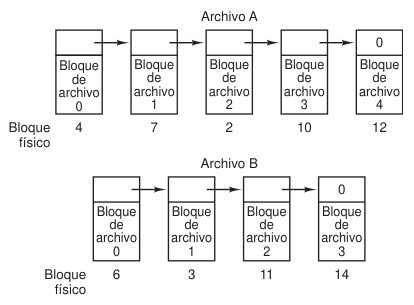
\includegraphics[width=0.7\linewidth]{imagenes/asign-lista-enlazada.png}
    \caption{Imagen sacada de \parencite{tanenbaum}. Almacenamiento de archivos como lista enlazada.}
    \label{fig:aign-lista-enlazada}
  \end{figure}

  Con este método no se pierde espacio debido a la fragmentación (salvo por la fragmentación interna del último bloque), y para acceder al archivo sólo hace falta saber la ubicación en disco del primer bloque. Sin embargo, el acceso aleatorio es super lento y, al tener que usar una parte del espacio de cada bloque para referenciar al siguiente, perdemos espacio de almacenamiento del archivo.

  \paragraph{Asignación de lista enlazada utilizando una tabla en memoria}\mbox{}\\
  Las dos desventajas de la asignación de lista enlzada se pueden eliminar si tomamos la palabra del puntero de cada bloque de disco y la ponemos en una tabla en memoria. En la Figura \ref{fig:asign-lista-enlazada-tabla} vemos un archivo A que utiliza los bloques de disco 4, 7, 2, 10 y 12, en ese orden y el archivo B que utiliza los bloques de disco 6, 3, 11 y 14, en ese orden.

  \begin{figure}[H]
    \centering
    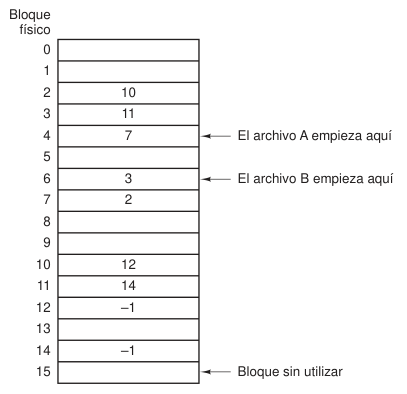
\includegraphics[width=0.5\linewidth]{imagenes/asign-lista-enlazada-tabla.png}
      \caption{Imagen sacada de \parencite{tanenbaum}.}
    \label{fig:asign-lista-enlazada-tabla}
  \end{figure}

  La principal desventaja de este método es que toda la tabla debe estar en memoria principal todo el tiempo para que funcione y esto es muy poco práctico.

  \paragraph{i-nodos}\mbox{}\\
  El último método que vamos a ver es el de asociar con cada archivo una estructura de datos conocida como \textbf{i-nodo}(\textbf{nodo-indice}), que lista los atributos y las direcciones de disco de los bloques del archivo. La gran ventaja de esto es que el i-nodo necesita estar en memoria sólo cuando está abierto el archivo correspondiente. Si cada i-nodo ocoupa $ n $ bytes, y puede haber un máximo de $ k $ archivos abiertos a la vez, la memoria total ocupada por el arreglo que contiente los i-nodos para los archivos abiertos es $ kn $ bytes.

  \begin{figure}[H]
    \centering
    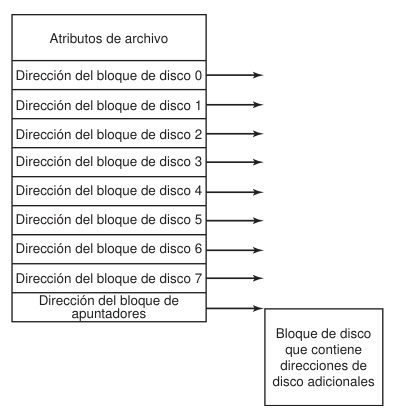
\includegraphics[width=0.5\linewidth]{imagenes/i-nodo.png}
    \caption{Imanen sacada de \parencite{tanenbaum}. Un i-nodo de ejemplo.}
    \label{fig:i-nodo}
  \end{figure}
  

  \subsubsection{Implementación de directorios}
  Cuando vamos a guardar un arhivo dentro de un directorio, tenemos dos posibilidades principales para almacenar los atributos de los mimsmo. Podemos almacenarlos directamente en la entrada del directorio, como se muestra en la Figura \ref{fig:almac-atrib-archivos} (a). Otra forma es almacenar los atributos en los i-nodos, en vez de hacerlo en la entrada de los directorios, como se muestra en la Figura \ref{fig:atributos-archivos}.

  \begin{figure}[H]
    \centering
    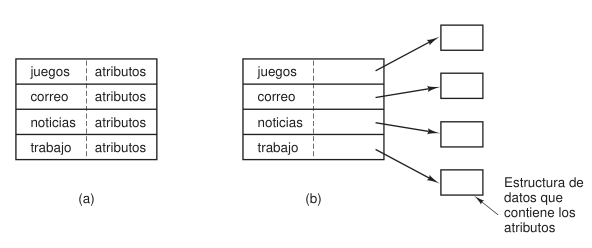
\includegraphics[width=0.8\linewidth]{imagenes/almac-atrib-archivos.png}
    \caption{Imagen sacada de \parencite{tanenbaum}. (a) Un directorio simple en Windows. (b) Un directorio en UNIX.}
    \label{fig:almac-atrib-archivos}
  \end{figure}

  Estas formas de almacenar los archivos son válidas pero traen problemas si queremos almacenar nombres de archivos mas largos, ya que la logitud de cada bloque es fija, por lo que los archivos que tengan nombres cortos estarían desperdiciando todo el espacio que les sobra.

  Una alternativa es que la estructura este dada en tres partes: una primera parte para indicar la longitud de la entrada, una segunda parte para almacenar los atributos, y la tercer parte continene el nombre del archivo, siendo este tan largo o corto como quiera el usuario. Esto se ve en la Figura \ref{fig:almac-nom-archivos} (a). Sin embargo esto trae problemas de fragmentación, aunque ahora es mas factible compactar el directorio ya que se encuentra en memoria principal.

  Otra manera de manejar los nombres de longitud variable es hacer que las entradas de directorio sean de longitud fija y mantener los nombres de los archivos juntos en un heap al final del directorio, como se muestra en la Figura \ref{fig:almac-nom-archivos} (b).

  \begin{figure}[H]
    \centering
    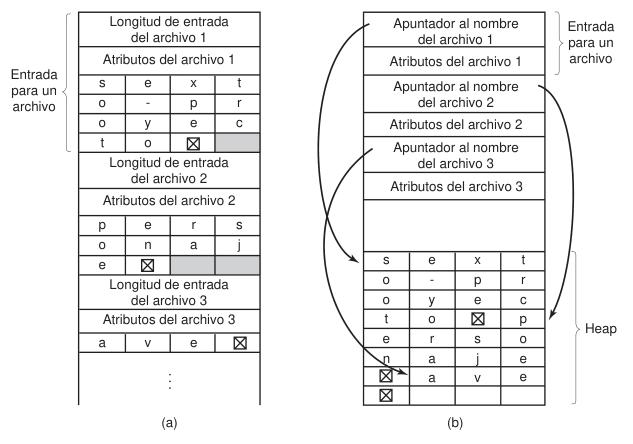
\includegraphics[width=0.9\linewidth]{imagenes/almac-nombres-archivos.png}
    \caption{Imagen sacada de \parencite{tanenbaum}. Dos maneras de manejar nombres de archivos de longitud variable. (a) En línea. (b) En un heap.}
    \label{fig:almac-nom-archivos}
  \end{figure}

  \subsubsection{Archivos compartidos}
  Cuando hay varios usuarios trabajando en conjunto en un proyecto, a menudo necesitan compartir archivos. De esta manera, resulta conveniente que un mismo archivo aparezca en dos directorios distintos (uno para cada usuario), como se vé en la Figura \ref{fig:archivo-compartido}. La conexión entre el directorio $ B $ y el archivo compartido del directorio $ C $ se conoce como \textbf{vínculo}. El sistema de archivos en sí ahora pasa a ser un \textbf{Grafo acíclico dirigido} (\textit{Directed Acyclic Graph}, \textbf{DAG}) en vez de un árbol.

  \begin{figure}[H]
    \centering
    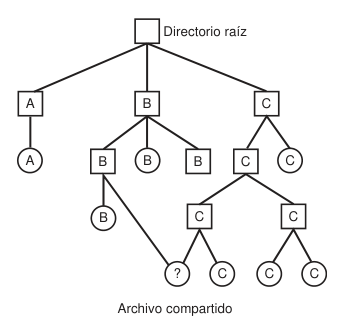
\includegraphics[width=0.5\linewidth]{imagenes/archivo-compartido.png}
    \caption{Imagen sacada de \parencite{tanenbaum}. Sistema que contiene un archivo compartido.}
    \label{fig:archivo-compartido}
  \end{figure}

  También existe lo que se conoce como \textbf{link simbólico} o \textbf{vínculo simbólico} en el que, al hacer el vínculo del directorio $ B $ a uno de los archivos de $ C $, el nuevo archivo (el que se crea como link en $ B $) contiene sólo el nombre de la ruta del archivo al cual está vinculado. 
  
  Ambos métodos tiene sus desventajas. En el caso de los \textit{hard-links} (los vínculos normales), supongamos el caso de la figura \ref{fig:archivo-compartido}. Si en algún momento el directorio $ C $ trata de eliminar el archivo que está vinculado con $ B $, el archivo va a seguir existiendo pero $ B $ será el único usuario con acceso al mismo, aunque el propietario sigue siendo $ C $ ya que no se puede eliminar el i-nodo del archivo en el que se encuentran los atributos (tampoco se puede modificar quién es el propietario). Entonces todos los cambios que haga $ B $ sobre el archivo se le van a acreditar a $ C $, muy probablemente quitándole espacio de almacenamiento por un archivo al que no puede acceder.

  Con los vínculos simbólicos no sucede esto ya que, como el archivo en $ B $ guarda la ruta del archivo en $ C $, si $ C $ elimina el archivo, la ruta que hay en $ B $ ya no es válida así que esta vez el archivo sí desaparece sin problemas. Sin embargo, la desventaja en este caso está en que cuando $ B $ quiere modificar el archivo se requiere de un mayor nivel de procesamiento ya que hay que leer la ruta del archivo a la que apunta, verificar si existe, ir hasta la ruta, acceder a su espacio en disco y recién ahí realizar los cambios requeridos.

  Existen muchos otros sistemas de archivos entre los que se encuentran: \textbf{Sistemas de archivos estructurados por registro}, \textbf{Sistemas de archivos por bitácora}, \textbf{Sistemas de archivos virtuales}. Estos últimos son sistemas de archivos que utiliza UNIX principalmente para poder integrar varios sistemas de archivos distintos en uno solo. 

  La mayoría de los sistemas UNIX utilizan el concepto de \textbf{VFS} (\textit{Virtual File System}) en el que todas las llamadas al sistema relacionadas con archivos se dirigen al sistema de archivos virtual para su procesamiento inicial. EStas llamadas, que provienen de procesos de usuarios, son las llamadas de POSIX estándar tales como \verb|open|, \verb|read|, \verb|write|, etc.

  \begin{figure}[H]
    \centering
    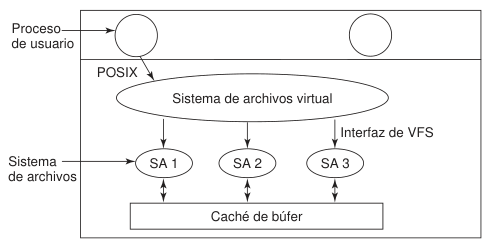
\includegraphics[width=0.7\linewidth]{imagenes/vfs.png}
    \caption{Imanen sacada de \parencite{tanenbaum}. Posición del sistema de archivos virtual.}
    \label{fig:vfs}
  \end{figure}

  \subsection{Administracion y optimizacion de sistemas de archivos}
  Siempre la idea de crear un sistema de archivos es hacerlo de manera eficiente. Por lo general los archivos se almacenan en disco, asi que la administracion del espacio en disco es una cuestion importante. Los puntos a tener en cuenta son:
  \begin{itemize}
    \item \textbf{Tamano de bloque.} Lo mas eficiente es almacenar los archivos en bloques de tamano fijo para evitar la fragmentacion del espacio. Es importante decidir el tamano que debe tener cada bloque ya que si se usan bloques de tamano muy grande, archivos de tamano pequeno desperdician el espacio. Por el contrario, si usamos bloques demasiado pequenos se pierde tiempo al leer los archivos.

    \item \textbf{Registro de bloques libres.} El siguiente paso es determinar c'omo llevar el regisro de los bloques libres. Se puede hacer de dos formas tambien: con una lista enlazada de bloques de disco, donde cada bloque contiene tantos numeros de bloques de disco libres como pueda. Con un bloque de 1 KB y un numero de disco de 32 bits, cada bloque en la lista de bloques libres contiene los numeros de 255 bloques libres (para un disco de 500 GB, se requieren aproximadamente 1.9 millones de bloques). La otra opcion es crear un mapa de bits, donde cada bit referencia a un bloque de disco. Si el bit es 0, el bloque esta libre, si el bit es 1 quiere decir que el bloque no esta vacio (para un disco de 500 GB ahora se necesitan aproximadamente 60.000 bloques).

    \item \textbf{Cuotas de disco.} Para evitar que los usuarios ocupen demasiado espacio en disco, los sistemas operativos multiusuario proporcionan un mecanismo para imponer las cuotas de disco.
  \end{itemize}

  \section{Unidad 4 - Administracion de Procesos}

  


  

  \newpage
  \addcontentsline{toc}{section}{Referencias}
  \printbibliography

\end{document}
